\documentclass{article}
\usepackage[paperwidth=511mm,paperheight=210mm,margin=0mm]{geometry}
\usepackage{fontspec}
\usepackage{xcolor}
\usepackage{contour}
\usepackage{graphicx}
\usepackage{tikz}
\pagestyle{empty}
\contourlength{1.8pt}
\setmainfont[Path=../tex/fonts/]{NanumMyeongjo.ttc}
\setsansfont[Path=../tex/fonts/]{NanumGothic.ttc}
\newfontfamily\coverdisplay{BM Yeonsung}
\definecolor{deepsea}{HTML}{062B4A}
\definecolor{cyansea}{HTML}{0B86A5}
\definecolor{paper}{HTML}{F7FBFA}
\begin{document}
\begin{tikzpicture}[x=1mm,y=1mm]
  % 새로 확장한 날개와 보존한 중앙 원본을 합친 전체 배경.
  \node[anchor=south west,inner sep=0] at (0,0)
    {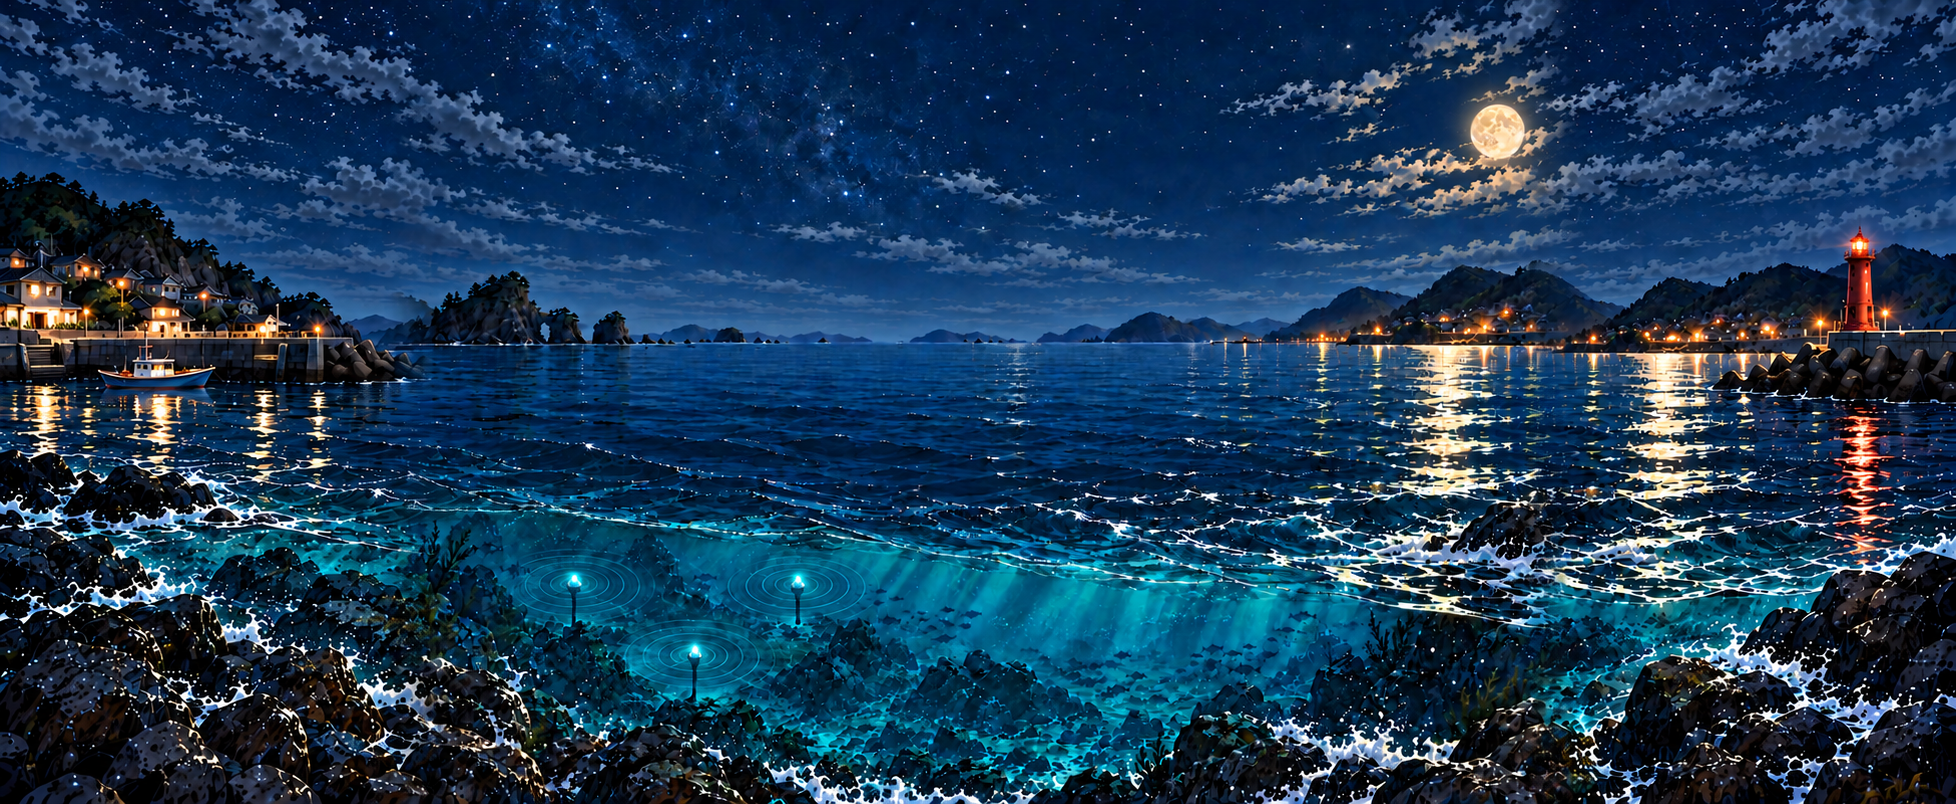
\includegraphics[width=511mm,height=210mm]{../images/cover-wrap-panorama-v11.png}};
  \fill[deepsea,opacity=.18] (0,0) rectangle (511,210);
  % 왼쪽 날개: 독자에게 건네는 짧은 안내
  \node[anchor=north west,text=white,align=left,text width=80mm] at (14,190)
    {\sffamily\bfseries\fontsize{15pt}{20pt}\selectfont 이 책을 펼치기 전에};
  \node[anchor=north west,text=white,align=left,text width=78mm] at (14,168)
    {\normalfont\fontsize{11pt}{17pt}\selectfont
    돌고래의 목소리는\par
    누구에게 먼저 닿을까요?\par\vspace{5mm}
    AI · 수중 마이크 · 해녀 ·\par
    바다 미스터리를 따라\par
    곰새코지의 밤으로\par
    함께 들어가 보세요.};
  \draw[white!45,line width=.4pt] (14,55) -- (86,55);
  \node[anchor=south west,text=white,align=left,text width=75mm] at (14,42)
    {\sffamily\fontsize{9pt}{13pt}\selectfont 초등 5–6학년 과학 모험 동화};

  % 뒷표지 문구
  \node[anchor=north west,text=white,align=left,text width=112mm] at (117,178)
    {\coverdisplay\fontsize{17pt}{22pt}\selectfont 새벽 세 시,\par 바다에서 이상한 신호가 잡혔다.};
  \node[anchor=north west,text=white,align=left,text width=112mm] at (117,150)
    {\coverdisplay\fontsize{12.2pt}{22pt}\selectfont
    제주 바닷가의 작은 마을 곰새코지.\par
    어느 새벽, 물마루 AI 연구소의 화면에\par
    낯선 문장이 떴다. 돌고래 소리를 분석한\par
    AI가 인간의 말로 바꾼 신호였다.\par\vspace{2mm}
    “돌려줘.”\par\vspace{2mm}
    누가, 무엇을 돌려 달라는 걸까?\par
    6학년 단우와 친구들은 수중 마이크 세 대의\par
    녹음, 관광선의 움직임, 해녀들의 바다 경험을\par
    하나씩 살핀다. 잘린 녹음 속 휘슬은 어디서\par
    왔는지, AI가 붙인 라벨은 믿을 만한지\par
    따라갈수록 새로운 의문이 생긴다.\par
    그러던 중 카메라 앞에 돌고래가\par
    불쑥 나타난다. 흩어진 소리와 기록을 이어\par
    붙인 아이들은 사라진 목소리의 진실을\par
    찾아낼 수 있을까?};

  % 책등도 같은 배경 위에 제목과 작가명만 얹어 별도 색 띠를 없앤다.
  \node[rotate=90,text=white,align=center] at (255.5,97)
    {\coverdisplay\fontsize{22.5pt}{25pt}\selectfont \contour{black}{곰새코지 돌고래 목소리 사건}};
  \node[rotate=90,text=white,align=center] at (255.5,34)
    {\coverdisplay\fontsize{9.5pt}{12pt}\selectfont \contour{black}{이희근}};

  % 앞표지 인물 그림을 연속 배경 위에 얹는다.
  \node[anchor=south,inner sep=0] at (337,4)
    {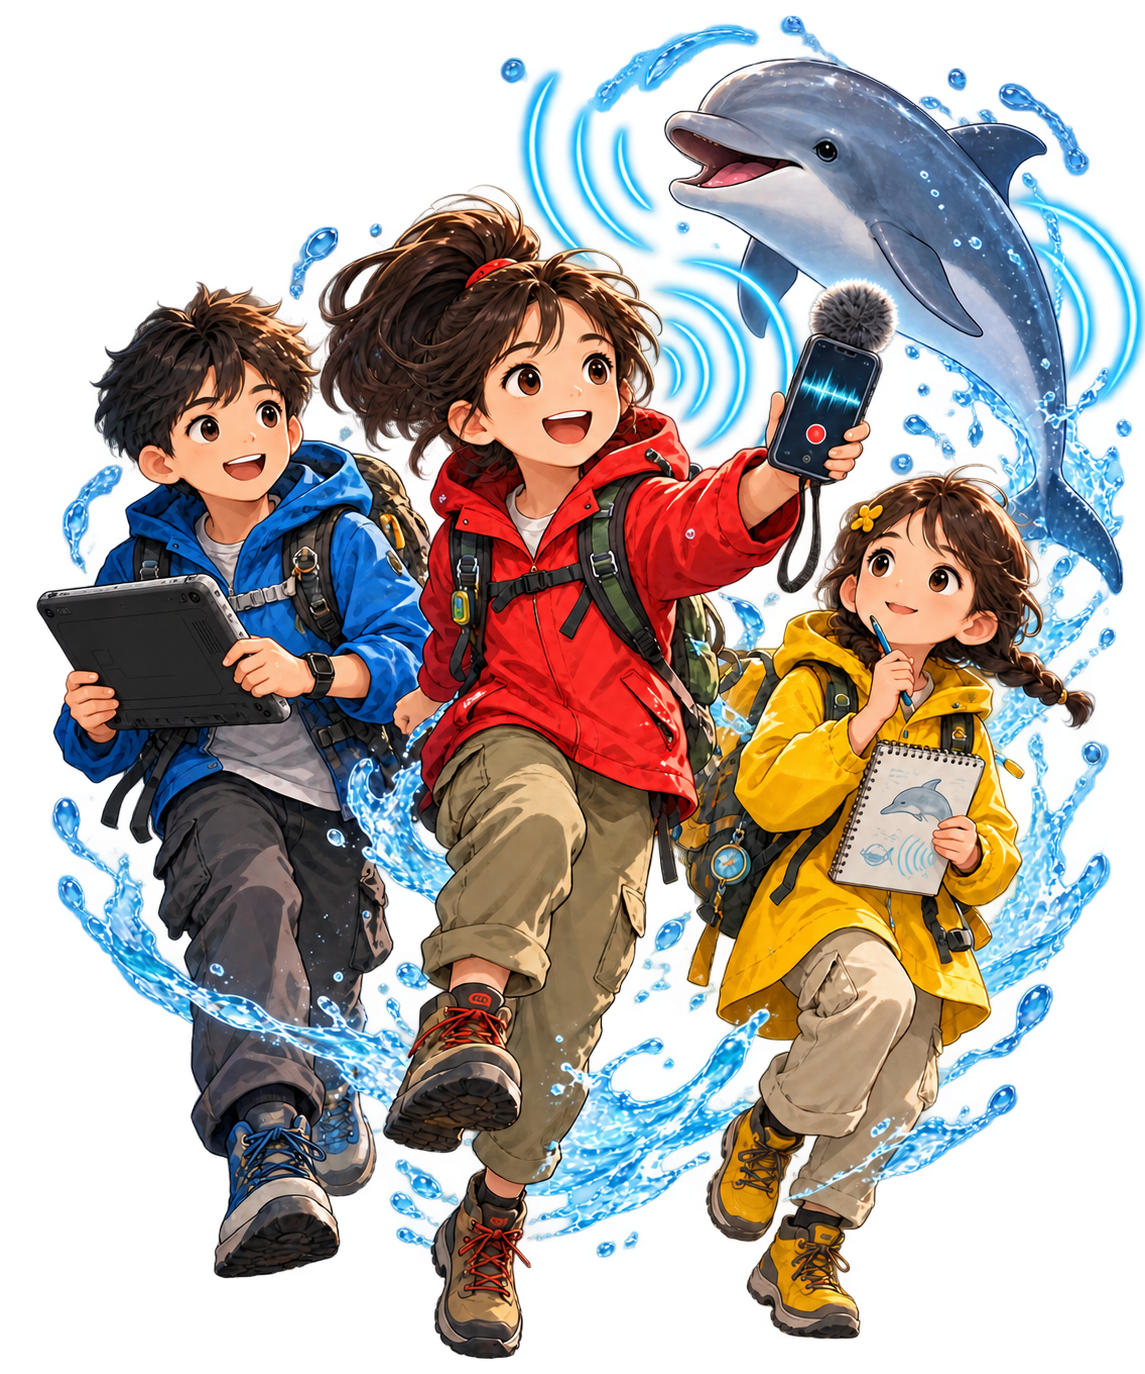
\includegraphics[width=109.6mm]{../images/title-adventure.png}};
  \node[anchor=north west,text=white,align=left,text width=120mm] at (283,191)
    {\sffamily\fontsize{10pt}{13pt}\selectfont 바다와 AI를 함께 읽는 과학 모험 이야기};
  \node[anchor=north,text=white,align=center,text width=134mm] at (328,174.1)
    {\coverdisplay\fontsize{40.8pt}{47pt}\selectfont
      \contour{black}{곰새코지 돌고래}\par
      \contour{black}{목소리 사건}};
  \node[anchor=north,text=white,align=center] at (342,127)
    {\coverdisplay\addfontfeatures{LetterSpace=8}\fontsize{10pt}{13pt}\selectfont 이희근};

  % 오른쪽 날개: 작가 및 독서 포인트
  \node[anchor=north west,text=white,align=left,text width=78mm] at (425,190)
    {\sffamily\bfseries\fontsize{14pt}{19pt}\selectfont 이 책의\par 탐사 키워드};
  \node[anchor=north west,text=white,align=left,text width=78mm] at (425,161)
    {\normalfont\fontsize{10pt}{15pt}\selectfont
    돌고래의 클릭음\par
    수중 마이크 세 대\par
    해녀의 바다 경험\par
    AI 라벨과 시민 과학};
  \draw[white!45,line width=.4pt] (425,90) -- (497,90);
  \node[anchor=north west,text=white,align=left,text width=76mm] at (425,78)
    {\sffamily\bfseries\fontsize{12pt}{16pt}\selectfont 작가의 말};
  \node[anchor=north west,text=white,align=left,text width=76mm] at (425,57)
    {\normalfont\fontsize{9pt}{14pt}\selectfont
    바다의 소리를 자세히 들으면\par
    과학과 상상이 만나는 순간이\par
    찾아옵니다.};
\end{tikzpicture}
\end{document}
